\documentclass[5p,letterpaper]{elsarticle}

\usepackage[T1]{fontenc}
\usepackage{newtxtext,newtxmath}
\usepackage{amsmath}
\usepackage{graphicx}
\usepackage{booktabs}
\usepackage{tabularx}
\usepackage{array}
\usepackage{xcolor}
\usepackage{enumitem}
\usepackage{microtype}
\usepackage[hidelinks]{hyperref}

\graphicspath{{figures/}}
\setlist{nosep,leftmargin=*}
\newcolumntype{L}{>{\raggedright\arraybackslash}X}
\newcommand{\cent}{\textcent}
\newcommand{\ind}{\mathbf{1}}

% many figures and tables: let them share pages with text instead of drifting to the end
\renewcommand{\topfraction}{0.9}
\renewcommand{\bottomfraction}{0.8}
\renewcommand{\textfraction}{0.07}
\renewcommand{\floatpagefraction}{0.8}
\renewcommand{\dbltopfraction}{0.9}
\renewcommand{\dblfloatpagefraction}{0.8}
\setcounter{topnumber}{3}
\setcounter{bottomnumber}{2}
\setcounter{totalnumber}{5}
\setcounter{dbltopnumber}{3}

% plain page numbers instead of the "Preprint submitted to" footer
\makeatletter
\def\ps@pprintTitle{\let\@oddhead\@empty\let\@evenhead\@empty
  \def\@oddfoot{\hfil\thepage\hfil}\let\@evenfoot\@oddfoot}
\makeatother

\begin{document}

\begin{frontmatter}

\title{Prediction Engine: single-market and cross-market arbitrage between Kalshi and Polymarket, and when a free lunch pays}

\author{Niclas Karlsen\corref{cor1}}
\ead{karlsenniclas@gmail.com}
\cortext[cor1]{Corresponding author.}
\affiliation{organization={Independent project},country={Norway}}

\begin{abstract}
Prediction markets list binary contracts that pay one dollar if an event happens. When the Yes and No sides of the same question can be bought for less than a dollar together, fees included, the difference is locked in whatever happens: a free lunch. This report documents Prediction Engine, a local tool that matches markets across Kalshi and Polymarket, walks both order books, charges each venue's fees and prices two kinds of arbitrage: buying both sides of one market on one venue (single-market) and buying Yes on one venue and No on the other (cross-market). An audit found sixteen faults, fourteen of them now fixed, after which an independent re-implementation agreed with the engine on all 736,856 values compared. A forward test swept all 363 matched pairs 22 times over 1.8 hours and priced every route for a \$1 bet and a \$1,000 bet. Single-market arbitrage never appeared: on both venues the two asks sum to a dollar plus the spread, and the lowest sum seen was 100.1 cents. Cross-market routes did turn positive after fees. Reading the settlement rules of the 28 flagged routes split them into 18 free lunches, which pay at least a dollar in every outcome, and 10 routes that are not sure bets, and the largest apparent edges belonged to the second group. On a \$1,000 bet the free lunches earned a median of 0.64 cents per one-dollar pair, 14 of 18 stayed positive in every sweep and 348 of 349 re-checks a minute later were still positive. Bet size cuts both ways. Kalshi rounds its fee up to the cent on every order, which cost a median 0.64 cents on a \$1 bet and turned six free lunches into losses; four of them, positive in every sweep at \$1,000, broke even after 2 to 6 contracts. Thin books worked the other way and cut the edge of seven free lunches on the larger bet. With settlement a median 75 days away, the annualised return was about 1.2\%: the free lunches are real, but small.
\end{abstract}

\begin{keyword}
Prediction markets \sep Arbitrage \sep Free lunch \sep Order books \sep Fee rounding \sep Kalshi \sep Polymarket
\end{keyword}

\end{frontmatter}

\section{Introduction}

A prediction market contract pays one dollar if an event happens and nothing otherwise, so its price can be read as the market's probability of the event \cite{wolfers2004}. Kalshi, a US exchange regulated by the Commodity Futures Trading Commission, and Polymarket, which runs a central limit order book with on-chain settlement, list many of the same questions: who wins a nomination, whether a company goes public, whether a central bank cuts rates.

Suppose Kalshi sells Yes on such a question for 60 cents and Polymarket sells No on the same question for 37 cents. Buying one of each costs 97 cents and pays exactly one dollar whichever way the question resolves, because one of the two contracts must win. The three cents do not depend on the outcome. If the two contracts cost 60 and 40 cents, the dollar paid out would only return the stake. This report calls a trade a \emph{free lunch} when the dollar it pays in every outcome is more than everything put in, fees included.

Three things get in the way. Fees are charged per contract, and Kalshi rounds its fee up to the cent on every order. The best quote is often only a few hundred contracts deep, so a larger order walks into worse prices. And two markets with almost the same title can settle on different events, deadlines or definitions, in which case the pair is not a hedge at all. The literature reflects all three. Saguillo et al.\ \cite{saguillo2025} define single-market and combinatorial arbitrage on Polymarket. Gebele et al.\ \cite{gebele2026executable} separate arbitrage in payoff space from what can actually be executed against the book. Cheng et al.\ \cite{cheng2026} find single-market arbitrage in NBA markets exceedingly rare, with seven executable in-game episodes and a median duration of 3.6\,s, while combinatorial opportunities were more common but limited by thin books. Gebele and Matthes \cite{gebele2026semantic} align equivalent markets across ten venues and report average price gaps of 2 to 4\%.

This project started from those papers. I built a tool that finds the same bet on Kalshi and Polymarket, prices both kinds of arbitrage at a size a person could actually trade, and shows the result clearly. The report then tests the tool on live markets. Its thesis is the following.

\medskip
\noindent\emph{Thesis.} Riskless arbitrage between Kalshi and Polymarket exists, but only across the two venues, only where both settle the same event, and only at a few tenths of a cent to two cents per dollar. Whether a trade captures it depends on its size: Kalshi's cent rounding can erase a sub-cent edge on a \$1 bet, while thin books can erode a larger edge on a \$1,000 bet.
\medskip

\noindent The report answers four research questions, each with hypotheses that the results either support or reject:
\begin{itemize}
\item \textbf{RQ1} (engine). Can a small local application match the same bet across the two venues and price arbitrage correctly at executable size?\\
\textbf{H1}: An independent re-implementation of the pricing reproduces every number the engine reports.
\item \textbf{RQ2} (single market). Can Yes and No of one market on one venue be bought for less than a dollar after fees?\\
\textbf{H2}: No. Both sides trade in one book, so the two asks sum to a dollar plus the spread, and fees only add to that.
\item \textbf{RQ3} (cross market). Do cross-market routes cost less than a dollar after fees, and how many of them are free lunches?\\
\textbf{H3}: Some cross-market routes stay below a dollar after fees and depth on a \$1,000 bet.\\
\textbf{H4}: The largest apparent edges come from pairs whose settlement rules differ, so they are not sure bets.\\
\textbf{H5}: The free lunches persist across sweeps, re-checks and the price history rather than being one-off glitches.
\item \textbf{RQ4} (bet size). How do fees, fee rounding and depth change a free lunch between a \$1 bet and a \$1,000 bet?\\
\textbf{H6}: Kalshi's cent rounding turns sub-cent free lunches into losses on a \$1 bet, and they pay once the bet passes a break-even size of a few contracts.\\
\textbf{H7}: The books are deep enough for a \$1,000 bet on most free lunches without losing the edge.
\end{itemize}

Section~\ref{sec:background} sets out the arbitrage conditions and the fees. Section~\ref{sec:system} describes the system and Section~\ref{sec:pricing} the pricing model. Section~\ref{sec:audit} reports the audit (RQ1). Section~\ref{sec:forward} presents a forward test over all matched pairs: single-market arbitrage (RQ2), cross-market arbitrage and the free lunches (RQ3), and the comparison of a \$1 bet with a \$1,000 bet (RQ4). Section~\ref{sec:discussion} evaluates the hypotheses and discusses the results and their limits, and Section~\ref{sec:conclusion} concludes.

\section{Background}\label{sec:background}

\subsection{Binary contracts and the one-dollar payout}

Each binary market has a Yes and a No contract. One of them pays a dollar at settlement, so a Yes and a No of the same market are worth exactly one dollar together. On both venues the two contracts share a single book: buying No at price $q$ is the same order as selling Yes at $1-q$. Kalshi's order-book endpoint returns bids only, so the engine derives the Yes ask as one minus the best No bid and the No ask as one minus the best Yes bid \cite{kalshibook}. Polymarket exposes the two outcome tokens as separate books, but its matching engine links them through minting and merging, so the same mirror holds. With $b_Y$ the best Yes bid and $a_Y, a_N$ the best asks, the No ask is $a_N = 1 - b_Y$, so
\begin{equation}\label{eq:mirror}
a_Y + a_N = a_Y + (1-b_Y) = 1 + (a_Y - b_Y) = 1 + s,
\end{equation}
where $s \ge 0$ is the bid-ask spread of the Yes book.

\subsection{Single-market arbitrage}

Following Cheng et al.\ \cite{cheng2026}, buying both outcomes of one market at the ask is profitable before fees when
\begin{equation}\label{eq:single}
a_Y + a_N < 1 .
\end{equation}
Saguillo et al.\ \cite{saguillo2025} call this long market rebalancing. Equation~(\ref{eq:mirror}) shows why it should not happen on a two-outcome market: the asks sum to one plus the spread, which is at least one tick while the book is not crossed, and fees only add to the cost. The mirror trade, minting a pair for a dollar and selling both sides at the bids, fails for the same reason, since $b_Y + b_N = 1 - s$. Single-market arbitrage can only appear in a crossed or stale book, or across the many outcomes of one event, which this two-leg tool does not price.

\subsection{Cross-market arbitrage and the free lunch}

Across venues the same test uses the Yes ask on one venue and the No ask on the other,
\begin{equation}\label{eq:cross}
a_Y^K + a_N^P < 1 ,
\end{equation}
with $K$ for Kalshi and $P$ for Polymarket, and the mirror route with the venues swapped. The two books are separate, so nothing ties their prices together except traders who buy on one venue and sell on the other.

Equation~(\ref{eq:cross}) only describes a riskless trade if both contracts refer to the same event. Let $A$ be the event that pays Kalshi Yes and $B$ the event that pays Polymarket Yes. Holding Kalshi Yes and Polymarket No pays
\begin{equation}\label{eq:payoff}
\Pi = \ind_A + \ind_{B^c} = 1 + \ind_{A\setminus B} - \ind_{B\setminus A},
\end{equation}
so the pair never pays less than a dollar if and only if $B \subseteq A$. When the two events are equal both routes pay exactly a dollar. When one is a strict subset of the other, only one direction is safe, and it pays two dollars in the outcome $A \setminus B$; the other direction loses both legs in that outcome. This report calls a route a \emph{free lunch} when it pays at least a dollar in every outcome and costs less than a dollar after fees at the size traded, and \emph{not a sure bet} when some outcome pays nothing on both legs. The settlement review in Section~\ref{sec:freelunch} applies this identity to every flagged pair.

\subsection{Fees and cent rounding}\label{sec:fees}

Kalshi charges a taker fee of $0.07 \times C \times P \times (1-P)$ for $C$ contracts at price $P$, rounded up to the next cent per order, with a multiplier for some series \cite{kalshifees}. Nearly every Kalshi snapshot in the forward test carried the rate 0.07. Polymarket charges takers $C \times r \times p \times (1-p)$ with a market-specific rate $r$ \cite{polyfees}, which was between 0.03 and 0.05 in most snapshots and 0.07 or zero in the rest. Both schedules peak at a price of 50 cents (Fig.~\ref{fig:fees}a).

The cent rounding is what makes bet size matter. The exact Kalshi fee on one contract is at most 1.75 cents, but the order pays at least one full cent and up to two. Near the edges of the price range the gap is largest: one contract at 99 cents owes 0.07 cents and pays a full cent (Fig.~\ref{fig:fees}b). On a large order the rounding is spread over every contract and disappears. Polymarket does not round, but its books reported a minimum order of 5 shares in every snapshot of the test, so the smallest cross-market bet both venues accept is about \$5.

Table~\ref{tab:stylised} runs the example from the introduction through both fee schedules, with Polymarket at a rate of 0.05. The 3-cent gap is a free lunch on a \$1,000 bet, but one, two or three contracts lose money, because the Kalshi leg pays 2, 4 and 6 cents of fees where 1.68, 3.36 and 5.04 cents are owed. From four contracts on the profit stays positive, and apart from a sawtooth of less than a cent it grows with the size of the bet.

\begin{figure}[tbp]
\centering
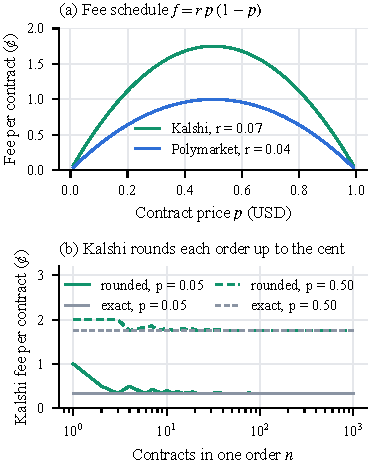
\includegraphics[width=\columnwidth]{fig_fees}
\caption{(a) Fee per contract on each venue. (b) Kalshi fee per contract with and without rounding each order up to the cent.}\label{fig:fees}
\end{figure}

\begin{table}[tbp]
\caption{A stylised free lunch, Kalshi Yes at 60 cents and Polymarket No at 37 cents ($r = 0.05$), at three bet sizes.}\label{tab:stylised}
\footnotesize
\begin{tabularx}{\columnwidth}{@{}Lrrr@{}}
\toprule
 & \$1 bet & 4 contracts & \$1,000 bet \\
\midrule
Kalshi Yes, 60\,\cent & \$0.60 & \$2.40 & \$600.00 \\
Polymarket No, 37\,\cent & \$0.37 & \$1.48 & \$370.00 \\
Kalshi fee, rounded up & \$0.02 & \$0.07 & \$16.80 \\
Polymarket fee & \$0.0117 & \$0.0466 & \$11.66 \\
Total stake & \$1.0017 & \$3.9966 & \$998.46 \\
Payout in every outcome & \$1.00 & \$4.00 & \$1,000.00 \\
\midrule
Profit & $-$\$0.0017 & \$0.0034 & \$1.54 \\
\bottomrule
\end{tabularx}
\end{table}

\section{System design}\label{sec:system}

Prediction Engine is a Python application with a browser interface, about 1,300 lines in total. Running \texttt{python main.py} starts the local server, opens the page in a browser and rescans both venues in the background when the market catalogue is missing or more than a day old. It uses only the public read-only endpoints of both venues, needs no API keys and never places orders. Fig.~\ref{fig:architecture} shows the structure. An offline scan builds a catalogue of matched pairs. The live part fetches order books when a user opens a bet, prices four routes and draws the charts.

\begin{figure*}[t]
\centering
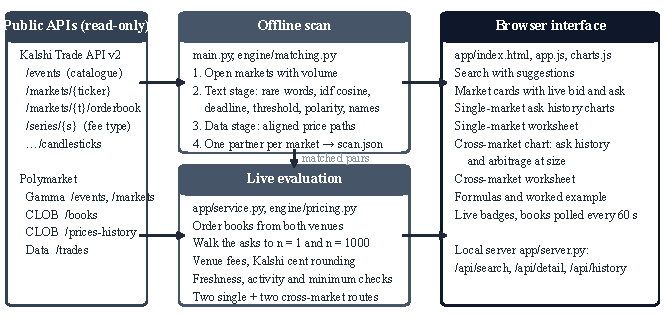
\includegraphics[width=0.95\textwidth]{fig_architecture}
\caption{System structure. The scan runs in the background and writes a catalogue; the live evaluation and the histories are computed per bet and served to the browser as JSON.}\label{fig:architecture}
\end{figure*}

\subsection{Catalogue scan and matching}

The scan downloads every open market with at least \$1,000 of volume: 27,109 on Kalshi and 9,728 on Polymarket in the final run. Matching has two stages (Fig.~\ref{fig:funnel}). The text stage tokenises titles, normalises numbers and dates, and keeps pairs that share a rare word or score at least 0.6 on an idf-weighted cosine. It then requires that deadlines, numeric thresholds, polarity (above or below, cut or hike, negation) and named people agree, and keeps the five closest candidates per Kalshi market. The data stage aligns the two price paths on an hourly or daily grid and accepts a pair when the paths are correlated and sit close together. Finally each market keeps only its best partner, because the runners-up are usually related bets whose gap merely looks like an edge. Of 234,918 text candidates, 431 passed the data stage and 363 remained as primary pairs.

\begin{figure}[tbp]
\centering
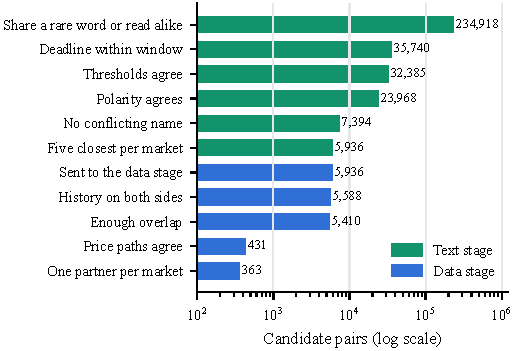
\includegraphics[width=\columnwidth]{fig_funnel}
\caption{Matching funnel of the final scan. Each bar counts the candidate pairs that pass the stage.}\label{fig:funnel}
\end{figure}

\subsection{Live evaluation}

When a bet is opened the engine fetches both order books and prices four routes: Yes and No on Kalshi, Yes and No on Polymarket, and the two cross-market routes. Each route is evaluated for one contract and for 1,000 contracts on each leg, which is a bet of about \$1 and about \$1,000, and at ten sizes in between for the depth chart. A result counts as an estimate only when both markets are active, both books arrived within 15\,s with less than 3\,s between them, the order meets the venue minimum and both fee rates are known. Cross-market results are always marked rules unverified, because price agreement does not prove that the markets settle alike.

\subsection{Ask histories}

Kalshi publishes candles with the Yes bid and ask for the whole life of a market, so its ask history is direct: the No ask is one minus the Yes bid. Polymarket only publishes a midpoint history, and Yes plus No midpoints sum to exactly one by construction. The engine therefore rebuilds a Polymarket ask path from the trades feed, as the volume-weighted price takers paid for each token per hour, in the spirit of the trade-based reconstruction in \cite{saguillo2025}. The feed serves the latest 11,000 trades, so busy markets have a shorter history. Each price is carried forward until the next one for at most a day, two for daily candles, after which the line breaks and no edge is drawn.

\subsection{Interface}

The browser page (Fig.~\ref{fig:ui}) has a search box with suggestions, a card per venue with live bid and ask, two single-market charts, worksheets for the single-market and cross-market routes with columns for one contract and for 1,000 contracts, a cross-market chart with an ask history and an arbitrage-at-size view, and a section that shows every formula with a worked example for the selected route. Fetched numbers are marked in the worked example so a reader can trace each result to its inputs. Books refresh every minute and a live badge on each chart shows the current Yes plus No cost.

\begin{figure*}[t]
\centering
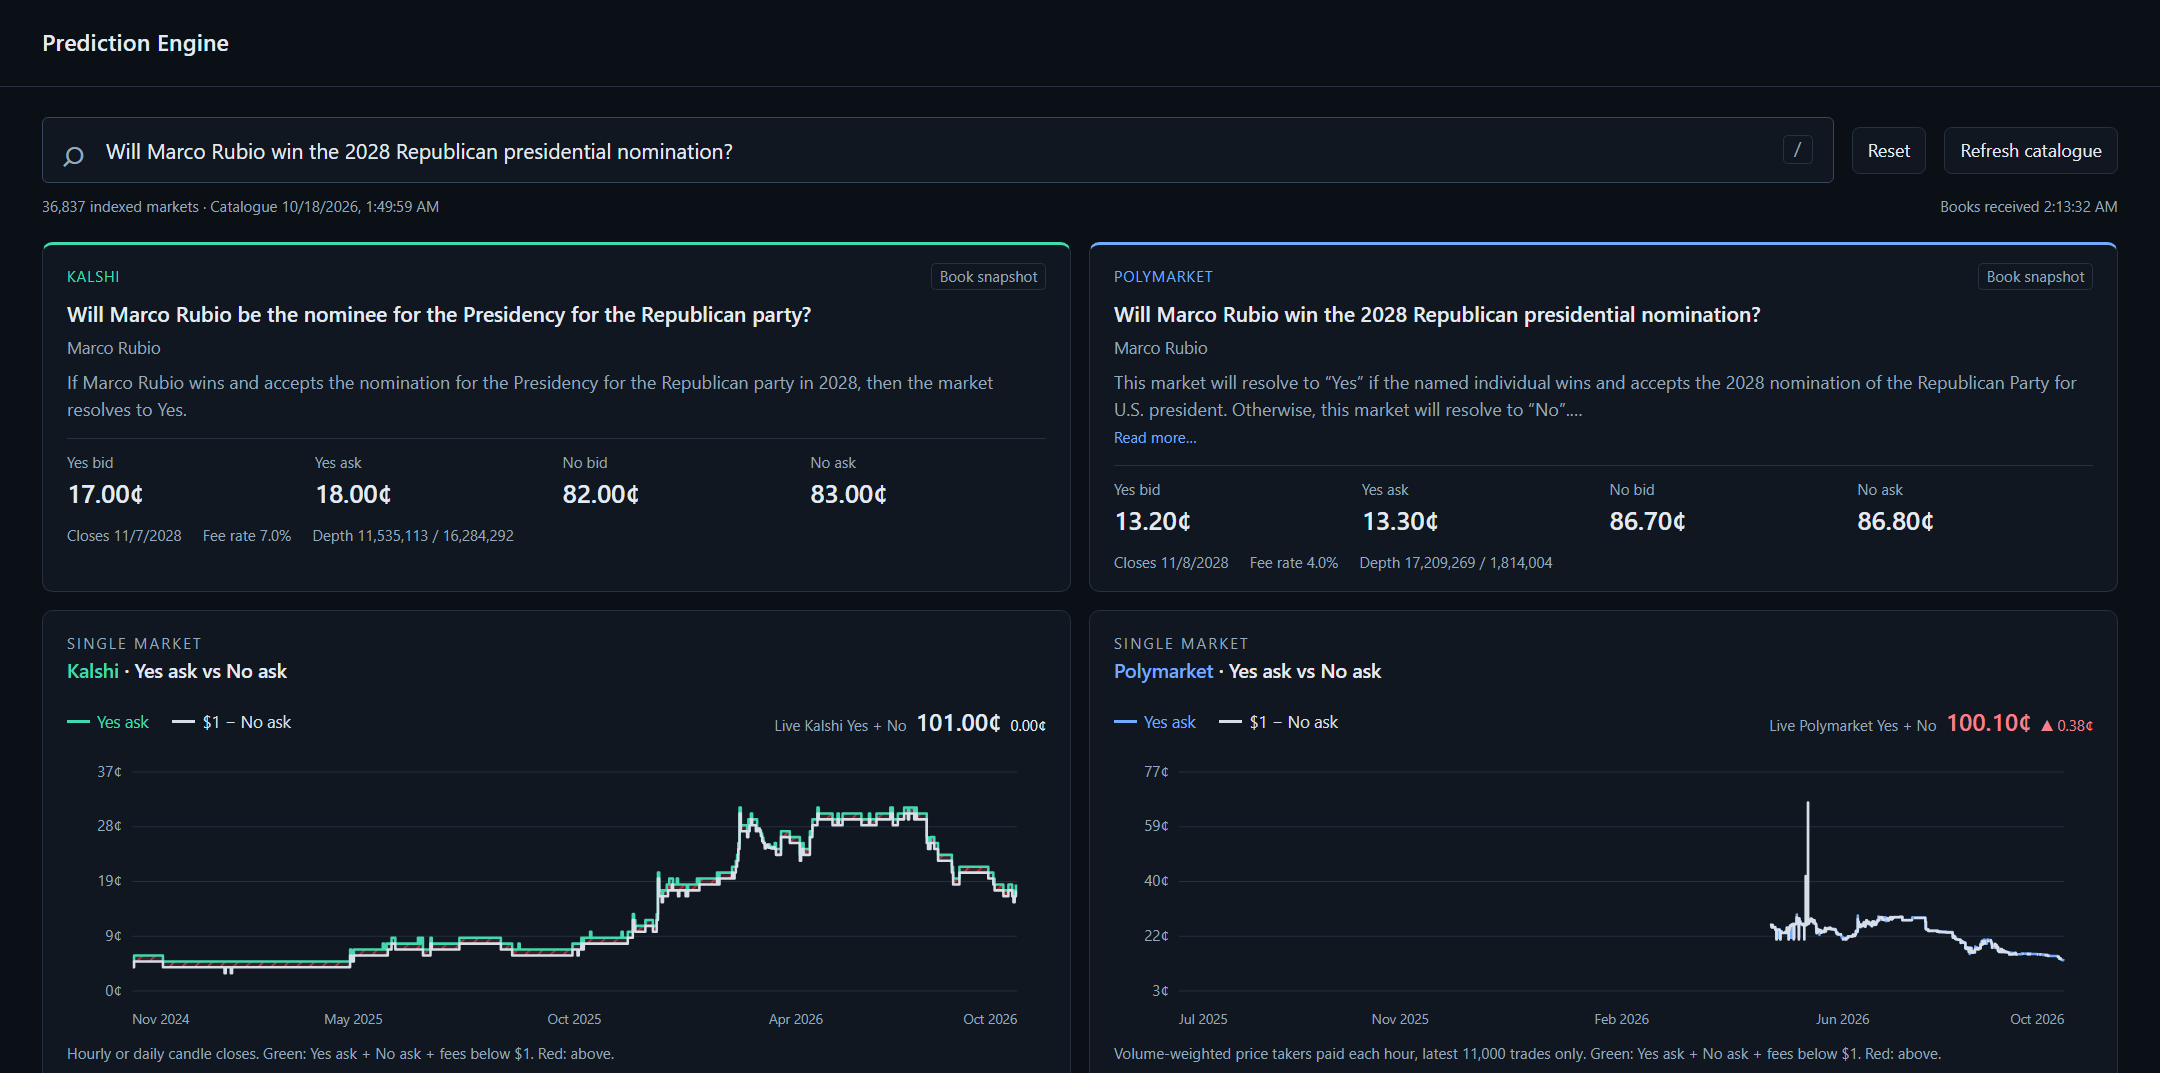
\includegraphics[width=0.92\textwidth]{ui_rubio_top}
\caption{The interface on the Marco Rubio nomination pair: venue cards with live quotes and the single-market charts. A hatched green fill marks hours when buying both legs plus fees cost less than a dollar, red when it cost more.}\label{fig:ui}
\end{figure*}

\section{Pricing model}\label{sec:pricing}

The engine follows the executable view of Gebele et al.\ \cite{gebele2026executable}: a quote is only worth what the book will fill. For an order of $N$ contracts on each leg, the executable size is set by the thinner book,
\begin{equation}\label{eq:size}
n = \min(N, Q_Y, Q_N),
\end{equation}
where $Q$ is the total depth of an ask book, rounded down to whole contracts when Kalshi is a leg. Each book is walked from the best price, which gives the acquisition cost and the fill price
\begin{equation}\label{eq:walk}
C(n) = \sum_i p_i q_i, \qquad \bar p = \frac{C(n)}{n}.
\end{equation}
The fee per leg is
\begin{equation}\label{eq:fee}
f = r \sum_i q_i\, p_i (1 - p_i),
\end{equation}
and Kalshi rounds it up to the cent, $f_K = \lceil 100 f \rceil / 100$. The cost of one pair and the net edge per pair are
\begin{equation}\label{eq:cost}
K = \bar p_Y + \bar p_N + \frac{f_Y + f_N}{n}, \qquad \pi = 1 - K .
\end{equation}
The profit locked in at settlement and the return on capital are
\begin{equation}\label{eq:profit}
\Pi = n \pi, \qquad \mathrm{ROI} = \frac{\pi}{K}.
\end{equation}
Slippage, $\bar p_Y + \bar p_N - a_Y - a_N$, is already inside the fill prices and is reported but not subtracted again. A return is annualised over the $D$ days to settlement as $(1+\mathrm{ROI})^{365/D} - 1$.

The rounding adds less than one cent to every Kalshi order, $0 \le f_K - f < 0.01$. Spread over a bet of $n$ pairs, it costs less than $1/n$ cents per pair, so with $\tilde\pi$ the edge before rounding in cents,
\begin{equation}\label{eq:breakeven}
\pi(n) > \tilde\pi(n) - \frac{1}{n} \quad\Rightarrow\quad \Pi(n) > 0 \text{ once } n \ge \frac{1}{\tilde\pi(n)} .
\end{equation}
A free lunch of 0.2 cents before rounding is therefore safe from five contracts on, while a one-contract bet can lose up to a cent per Kalshi order. The single-market route on Kalshi places two Kalshi orders and pays the rounding twice. Table~\ref{tab:notation} summarises the notation.

\begin{table}[tbp]
\caption{Notation.}\label{tab:notation}
\footnotesize
\begin{tabularx}{\columnwidth}{@{}lL@{}}
\toprule
Symbol & Meaning \\
\midrule
$a_Y, a_N$; $b_Y, b_N$ & Best ask and best bid of the Yes and No leg \\
$s$ & Bid-ask spread of the Yes book \\
$N$, $n$ & Contracts ordered, contracts filled on each leg \\
$Q$ & Total depth of an ask book \\
$C(n)$, $\bar p$ & Acquisition cost and fill price of one leg \\
$r$, $f$ & Fee rate and fee of one leg \\
$K$, $\pi$, $\tilde\pi$ & Cost and net edge of one pair, edge before rounding \\
$\Pi$, ROI & Profit at settlement and return on capital \\
$A$, $B$ & Events that pay Kalshi Yes and Polymarket Yes \\
\bottomrule
\end{tabularx}
\end{table}

\section{Audit}\label{sec:audit}

\subsection{Method}

The audit combined four checks. First, an independent reviewer read every code path for correctness, with the instruction to report only faults it could reproduce. Second, I probed the live APIs to test assumptions the code relies on, for example what a timestamp means or whether every record carries the fields the parser expects. Third, I re-implemented the pricing of Section~\ref{sec:pricing} from scratch and compared it with the engine. Fourth, after fixing faults I ran the scan, the server and the browser end to end on a fresh catalogue. Table~\ref{tab:audit} lists the findings.

\begin{table*}[t]
\caption{Audit findings, ranked by severity.}\label{tab:audit}
\footnotesize
\begin{tabularx}{\textwidth}{@{}lllLl@{}}
\toprule
ID & Severity & Component & Fault and consequence & Status \\
\midrule
A1 & High & Kalshi and Polymarket clients & One market without a title (1 of 144,593 Kalshi records) raised an exception that aborted the whole catalogue scan. & Fixed \\
A2 & High & Pair selection & The app fell back to pairs the scan had rejected under one partner per market; 68 of 87 such pairs were reachable, e.g.\ Pahlavi recognised as leader vs Pahlavi entering Iran. & Fixed \\
A3 & Medium & Freshness check & The Polymarket book timestamp is the time of the last change, not of the response, so quiet books failed the 15\,s check and every Polymarket route read as unverified. & Fixed \\
A4 & Medium & Polymarket catalogue & 19 markets listed under two events were counted twice, doubling title similarity (up to 1.51) and opening the 120-day deadline window. & Fixed \\
A5 & Medium & Polymarket ask history & Hourly buckets were labelled at the start of the hour while Kalshi candles are labelled at the end, a one-hour look-ahead in the cross-market chart. & Fixed \\
A6 & Medium & Rate-limit backoff & Three short retries gave up under load; the first fresh scan lost one side of the history for 1,460 of 5,947 candidates. & Fixed \\
A7 & Medium & Price-path matcher & The level-ratio test rejects true pairs at low prices: 145 candidates failed on the ratio alone, among them the US aliens pair (ratio 1.303). & Open \\
A8 & Medium & Deadline window & Titles that read as the same sentence may differ by up to 120 days in deadline, which let a Dec 1 market pair with a Dec 31 market. & Open \\
A9 & Low & Tokeniser & A title containing ``\#.'' raised a ValueError that aborted the scan. & Fixed \\
A10 & Low & History cache & A narrow exception filter and a shared temporary file let one bad history or two concurrent writers abort a scan. & Fixed \\
A11 & Low & Route status & A venue error was reported as ``No liquidity''. & Fixed \\
A12 & Low & Browser polling & A failed refresh was silent, and the depth chart kept old curves after a refresh. & Fixed \\
A13 & Low & Browser history & Refresh books never retried a history load that had failed. & Fixed \\
A14 & Low & Thread pools & Slow history jobs shared a pool with live books and could delay a book beyond the 3\,s skew limit. & Fixed \\
A15 & Low & Catalogue swap & A rescan replaced the catalogue one attribute at a time, so a request mid-swap could mix two catalogues. & Fixed \\
A16 & Low & Repository & Compiled \texttt{\_\_pycache\_\_} files were tracked in the initial commit. & Fixed after the test \\
\bottomrule
\end{tabularx}
\end{table*}

\subsection{The faults that mattered most}

Finding A1 was found by running a fresh scan rather than by reading code. One Kalshi market, a model release question, arrived without a title field, and the strict dictionary lookup aborted a scan of more than 144,000 records. The fix falls back to the event title. Finding A2 was the most serious for trading. The scan deliberately keeps one partner per market, but the app looked up any accepted pair, so it offered related but different bets as arbitrage. Restricting selection to primary pairs removed every one of the pairings the reviewer listed.

Finding A3 came from a probe: two requests for the same Polymarket book 3.8\,s apart returned timestamps that had aged by exactly 3.8\,s. The timestamp marks the last change of the book, so the freshness rule rejected books that were simply quiet. Freshness is now judged on when the book was received. Finding A6 showed up as a difference between two scans: the first fresh scan confirmed 341 pairs, the second, with warm caches, 431. The difference was rate limiting during the history stage, and longer backoff closed it.

Findings A7 and A8 are left open on purpose. The matcher was tuned on a hand-labelled sample that is not part of the repository, and changing its thresholds without that sample would trade one error for another. Both are discussed with a proposed fix in Section~\ref{sec:limitations}. Finding A16 was closed after the test with a \texttt{.gitignore}.

\subsection{Verification after the fixes}

The re-implemented pricing was compared with the engine on every snapshot of the forward test: 8,556 snapshots, four routes, four order sizes and six quantities each, 736,856 values in total, with 0 mismatches. The checks that the reviewer also confirmed as correct include the fee formulas against both venues' documentation, the ask derivation from Kalshi bids, the orientation of inverted pairs, time units, and the escaping of all text from the APIs before it reaches the page. The fixes raised the number of primary pairs from 291 in the first run to 363 in the final run.

\section{Forward test}\label{sec:forward}

\subsection{Protocol}

Starting at 23:50 UTC on 17 October 2026, a test harness swept all 363 primary pairs every five minutes, 22 times in total, over 1.8 hours. Each sweep fetched both books for every pair through the engine's own client code and stored the raw ask ladders, enough levels to fill 1,000 contracts, so every number below can be recomputed. A pair whose best route looked positive was fetched again after the sweep, a median of 62\,s later, to see whether the edge survived about the length of the app's refresh interval. No orders were placed.

Every route is priced for three bets. A \emph{\$1 bet} buys one contract on each leg; a pair costs just under a dollar, so this is the smallest bet that can capture a free lunch. A \emph{\$5 bet} buys five contracts, the smallest order Polymarket accepts. A \emph{\$1,000 bet} buys 1,000 contracts on each leg, which cost between \$977 and \$1,002 for the free lunches. On Polymarket a \$1 bet is below the minimum order, so the \$1 column shows what fees and books would give such a bet; the \$5 bet is the smallest that can actually be placed. A paper trade was recorded once per episode, at the first sweep in which a route was positive at \$1,000, and priced at all three sizes from the same books.

\subsection{Single-market arbitrage}

No single-market route was ever cheaper than a dollar before fees: the lowest Yes plus No ask on Kalshi was 100.10 cents and on Polymarket 100.10 cents (Fig.~\ref{fig:topsum}). That is Eq.~(\ref{eq:mirror}) at work, one tick of spread above a dollar. After fees not one of the 6,489 priced Kalshi snapshots and 7,393 priced Polymarket snapshots was positive, for a \$1 bet or a \$1,000 bet (Table~\ref{tab:routes}). The best Kalshi route lost 1.00 cent per pair on a \$1 bet and 0.22 cents on a \$1,000 bet; the best Polymarket route lost 0.10 cents at both sizes. The median Kalshi route lost 5.0 cents on a \$1 bet, of which a median 1.15 cents was the rounding on its two orders, and 7.5 cents on a \$1,000 bet, where the walk reaches deeper and wider levels. Single-market arbitrage did not occur, which matches the rarity reported in \cite{cheng2026}.

\begin{figure}[tbp]
\centering
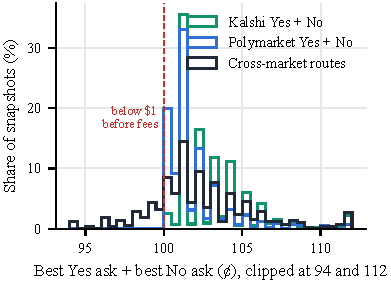
\includegraphics[width=\columnwidth]{fig_topsum}
\caption{Best Yes ask plus best No ask over all snapshots. Single-market routes never fall below 100 cents; only cross-market routes do.}\label{fig:topsum}
\end{figure}

\begin{table}[tbp]
\caption{Route statistics over all sweeps. The last two columns count snapshots that were still positive after fees and depth.}\label{tab:routes}
\footnotesize
\begin{tabularx}{\columnwidth}{@{}Lrrrr@{}}
\toprule
Route & Priced & Asks $<$ \$1 & \$1 bet & \$1,000 bet \\
\midrule
Kalshi Yes + No & 6,489 & 0 & 0 & 0 \\
Polymarket Yes + No & 7,393 & 0 & 0 & 0 \\
Kalshi Yes + Poly No & 7,303 & 954 & 343 & 198 \\
Poly Yes + Kalshi No & 6,577 & 1,537 & 678 & 372 \\
\bottomrule
\end{tabularx}
\par\smallskip\raggedright Counts are snapshots; a pair contributes once per sweep.
\end{table}

\begin{figure*}[t]
\centering
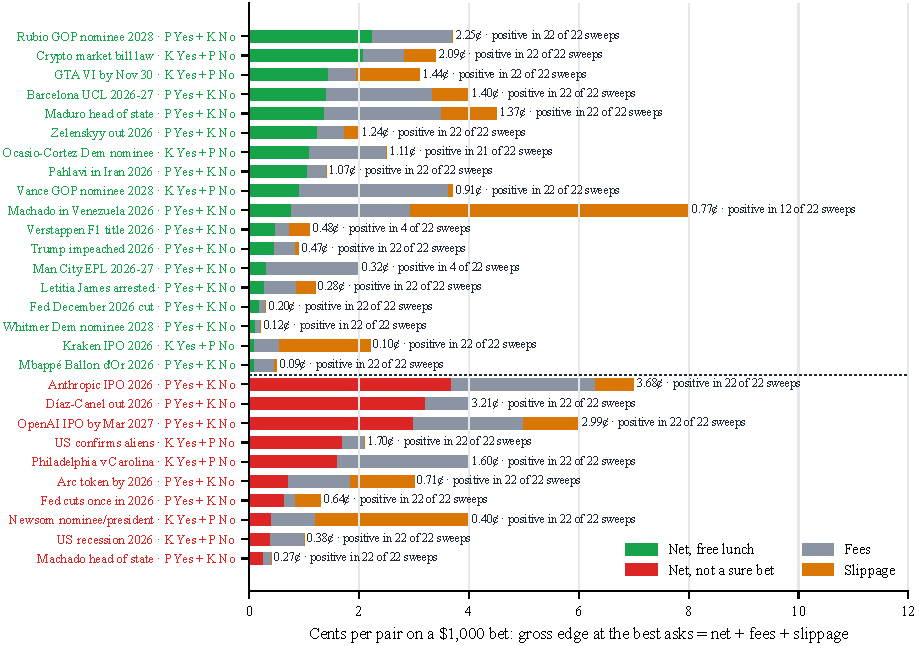
\includegraphics[width=\textwidth]{fig_waterfall}
\caption{Every route flagged during the test, split into free lunches (top, green) and routes that are not sure bets (bottom, red). Each bar decomposes the gross edge at the best asks into the net edge on a \$1,000 bet, fees and slippage, at the route's best sweep.}\label{fig:waterfall}
\end{figure*}

\begin{table*}[t]
\caption{Routes that are not sure bets and why. Net edges are medians over the sweeps.}\label{tab:notsure}
\footnotesize
\begin{tabularx}{\textwidth}{@{}lLlrr@{}}
\toprule
Pair and route & How the settlement differs & Relation of the events & \$1 bet (\cent) & \$1,000 bet (\cent) \\
\midrule
Anthropic IPO 2026 $\cdot$ P Yes + K No & Kalshi: IPO confirmed; Polymarket: shares listed and trading & Polymarket Yes $\subset$ Kalshi Yes & 4.01 & 3.66 \\
D\'iaz-Canel out 2026 $\cdot$ P Yes + K No & Kalshi: First Secretary of the party; Polymarket: President of Cuba & different office & 3.00 & 3.21 \\
OpenAI IPO by Mar 2027 $\cdot$ P Yes + K No & Kalshi: IPO confirmed; Polymarket: IPO completed & Polymarket Yes $\subset$ Kalshi Yes & 3.34 & 2.99 \\
US confirms aliens $\cdot$ K Yes + P No & Kalshi before Dec 1, Polymarket by Dec 31 & Kalshi Yes $\subset$ Polymarket Yes & 0.91 & 1.70 \\
Philadelphia v Carolina $\cdot$ K Yes + P No & Philadelphia wins vs Panthers cover $-2.5$ & moneyline vs spread & 1.26 & 1.60 \\
Fed cuts once in 2026 $\cdot$ P Yes + K No & Kalshi counts decisions, Polymarket counts 25\,bp steps & Polymarket Yes $\subset$ Kalshi Yes & 0.25 & 0.61 \\
Newsom nominee/president $\cdot$ K Yes + P No & Kalshi: both nominations; Polymarket: Newsom wins the presidency & different event & 2.68 & 0.40 \\
US recession 2026 $\cdot$ K Yes + P No & Polymarket also counts an NBER announcement & Kalshi Yes $\subset$ Polymarket Yes & $-0.28$ & 0.38 \\
Machado head of state $\cdot$ P Yes + K No & Kalshi de facto, Polymarket officially holds & de facto vs official & $-0.62$ & 0.27 \\
Arc token by 2026 $\cdot$ P Yes + K No & Polymarket requires a tradable governance token & Polymarket Yes $\subset$ Kalshi Yes & 1.48 & 0.14 \\
\bottomrule
\end{tabularx}
\par\smallskip\raggedright The Machado head of state book held only 9 contracts, so its \$1,000 bet fills \$8.98.
\end{table*}

\subsection{Cross-market arbitrage}

Cross-market routes behaved differently, because nothing but other traders ties two venues' books together. Of 13,880 priced cross-market snapshots, 2,491 had best asks summing to less than a dollar, 1,021 were still positive after fees on a \$1 bet and 570 on a \$1,000 bet (Table~\ref{tab:routes}). A gap at the best asks is therefore a weak signal: three in four disappear once fees and depth are counted. More snapshots survive at \$1 than at \$1,000 across the whole sample, because many gaps sit on a top level only a few contracts deep. Over the whole test 28 distinct cross-market routes were positive at \$1,000 and passed every validity check in at least one sweep.

\begin{figure}[tbp]
\centering
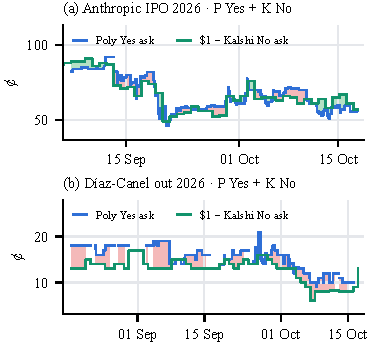
\includegraphics[width=\columnwidth]{fig_notsure_history}
\caption{Ask histories of the two largest routes that are not sure bets. A history like this cannot reveal a settlement mismatch; only the rules can.}\label{fig:notsure}
\end{figure}

\subsection{Free lunches and bets that only look safe}\label{sec:freelunch}

For each of the 28 routes I read both venues' settlement rules and applied the identity in Eq.~(\ref{eq:payoff}). A route is a free lunch when the two markets settle on the same event, or when the flagged direction is the safe one of a subset pair, so that it pays at least a dollar in every outcome. It is not a sure bet when some outcome pays nothing on both legs. The review gave 18 free lunches and 10 routes that are not sure bets (Fig.~\ref{fig:waterfall}).

The split is not a detail. On a \$1,000 bet the not-sure bets had a median net edge of 1.10 cents per pair against 0.64 cents for the free lunches, and the largest apparent edge of the whole test, 3.68 cents on Anthropic IPO 2026 at its best sweep, belonged to them. Table~\ref{tab:notsure} shows why. The Anthropic and OpenAI pairs compare a company confirming an IPO with the IPO taking place. The US aliens pair compares a deadline of 1 December with one of 31 December. A football pair compares a moneyline with a points spread. In each case the price gap is real but the hedge is not: there is an outcome in which both legs expire worthless. Their price histories look just as convincing as those of the free lunches (Fig.~\ref{fig:notsure}), which is why the rules, and not the data, decide. Fig.~\ref{fig:uicross} in the appendix shows how the engine itself presents one of them: the US aliens route is a positive estimate labelled rules unverified, and only the rules reveal that a confirmation during December would make both legs worthless.

\subsection{A \$1 bet against a \$1,000 bet}\label{sec:betsize}

Fig.~\ref{fig:bars} prices every free lunch at the three bet sizes. The median net edge per pair was 0.83 cents on a \$1 bet, 0.97 cents on a \$5 bet and 0.64 cents on a \$1,000 bet, but the medians hide two opposite effects.

The first is the cent rounding. On a \$1 bet it cost the free lunches a median 0.64 cents per pair, as much as the median free lunch earns on a \$1,000 bet, and up to 0.94 cents. Six of the 18 free lunches lost money on a \$1 bet. Four of them, Trump impeached 2026, Fed December 2026 cut, Whitmer Dem nominee 2028 and Mbapp\'e Ballon d'Or 2026, were positive on a \$1,000 bet in every one of the 22 sweeps. They broke even after 2, 4, 6 and 6 contracts, well within the bound of Eq.~(\ref{eq:breakeven}) for edges of 0.1 to 0.5 cents before rounding, and from there the profit grew with the size of the bet. Whitmer and Mbapp\'e still lost money at the 5-share minimum. The routes hit hardest have a Kalshi leg priced at 96 cents or more, where the exact fee is a small fraction of a cent but the order still pays a full one. Fig.~\ref{fig:curve} shows the effect contract by contract, and Table~\ref{tab:worked} follows the Fed route through it: the same books give a loss of 0.73 cents on a \$1 bet and a profit of \$1.95 on a \$1,000 bet.

The second effect is depth. Seven free lunches earned at least 0.3 cents more per pair on a \$5 bet than on the \$1,000 bet, because the best prices did not reach 1,000 contracts. Machado in Venezuela 2026 earned 5.65 cents per pair on a \$5 bet and 0.15 cents on a \$1,000 bet; Kraken IPO 2026 fell from 1.55 to 0.06 cents and Crypto market bill law from 2.57 to 1.04 cents. The Machado curve in Fig.~\ref{fig:curve} shows how: the trade earns money on each contract while the Yes ask lies below one minus the No ask, less fees, and that gap closes after a few hundred contracts as the walk leaves the best prices. Every free lunch still had at least 1,000 contracts on both legs, and 16 of the 18 were profitable on the \$1,000 bet in the median sweep.

The money follows the size of the bet, not the edge per dollar. The 18 free lunches together earned \$122.41 on \$1,000 bets in the median sweep, while the same trades as \$1 bets would have earned about 15 cents. Table~\ref{tab:ledger} compares the paper trades. A naive rule that trusts any best-ask sum below a dollar fires 2,491 times, but only 570 of those survive fees and depth at \$1,000. Following the engine alone opens 31 paper trades. Restricted to free lunches, 13 of 21 trades made money as \$1 bets, 19 as \$5 bets and all 21 as \$1,000 bets, for \$146.41 of locked profit on \$20,853.59 of capital. The review removes the trades with the highest returns, which is exactly the pattern one expects when the largest gaps are priced risk rather than mistakes.

\begin{figure}[tbp]
\centering
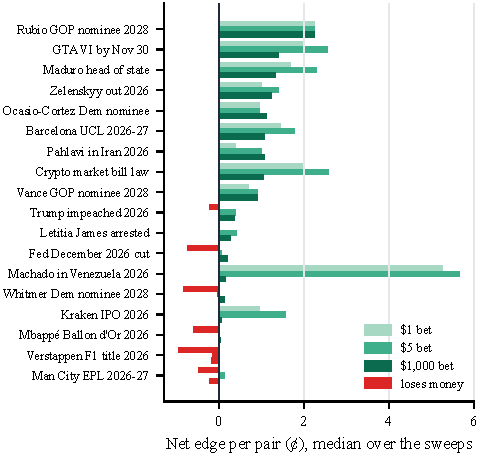
\includegraphics[width=\columnwidth]{fig_bet_bars}
\caption{Net edge per pair of every free lunch on a \$1 bet, a \$5 bet and a \$1,000 bet, median over the sweeps. Red bars lose money.}\label{fig:bars}
\end{figure}

\begin{figure}[tbp]
\centering
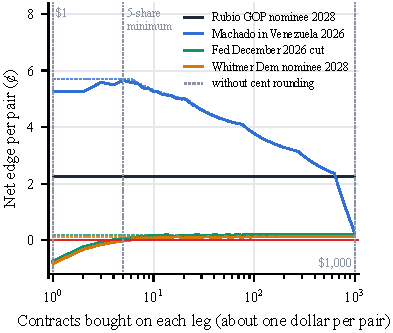
\includegraphics[width=\columnwidth]{fig_bet_curve}
\caption{Net edge per pair against contracts bought, at the median sweep of four free lunches. Solid lines include Kalshi's cent rounding, dashed lines leave it out. Rounding pulls the Fed and Whitmer routes below zero on small bets; depth pulls the Machado route down on large ones.}\label{fig:curve}
\end{figure}

\begin{table}[tbp]
\caption{Two free lunches at a \$1 bet and a \$1,000 bet, priced from the same books (median sweep). Both routes buy Polymarket Yes and Kalshi No.}\label{tab:worked}
\footnotesize
\setlength{\tabcolsep}{3.5pt}
\begin{tabularx}{\columnwidth}{@{}Lrrrr@{}}
\toprule
 & \multicolumn{2}{c}{Rubio GOP 2028} & \multicolumn{2}{c}{Fed Dec 2026 cut} \\
\cmidrule(lr){2-3}\cmidrule(lr){4-5}
 & \$1 & \$1,000 & \$1 & \$1,000 \\
\midrule
Fill price, Yes leg (\cent) & 13.30 & 13.30 & 0.70 & 0.70 \\
Fill price, No leg (\cent) & 83.00 & 83.00 & 99.00 & 99.00 \\
Polymarket fee per pair (\cent) & 0.46 & 0.46 & 0.03 & 0.03 \\
Kalshi fee per pair (\cent) & 1.00 & 0.99 & 1.00 & 0.07 \\
Cost per pair $K$ (\cent) & 97.76 & 97.75 & 100.73 & 99.80 \\
Net per pair $\pi$ (\cent) & 2.24 & 2.25 & $-0.73$ & 0.20 \\
Stake & \$0.98 & \$977.49 & \$1.01 & \$998.05 \\
Locked profit & \$0.02 & \$22.51 & $-$\$0.01 & \$1.95 \\
ROI & 2.29\% & 2.30\% & $-0.73$\% & 0.20\% \\
\bottomrule
\end{tabularx}
\end{table}

\begin{table}[tbp]
\caption{Paper-trading ledger, one trade per episode, priced at three bet sizes.}\label{tab:ledger}
\footnotesize
\setlength{\tabcolsep}{3.5pt}
\begin{tabularx}{\columnwidth}{@{}Lrrrrr@{}}
\toprule
Strategy & Bet & Trades & Won & Profit & ROI \\
\midrule
Best-ask sum below \$1 & & 2,491 & & -- & -- \\
\addlinespace
Engine signal & \$1 & 31 & 21 & \$0.30 & 0.96\% \\
 & \$1,000 & 31 & 31 & \$298.30 & 1.00\% \\
\addlinespace
\quad of which not sure bets & \$1,000 & 10 & 10 & \$151.89 & 1.71\% \\
\addlinespace
Engine signal and review & \$1 & 21 & 13 & \$0.14 & 0.65\% \\
 & \$5 & 21 & 19 & \$1.19 & 1.14\% \\
 & \$1,000 & 21 & 21 & \$146.41 & 0.70\% \\
\bottomrule
\end{tabularx}
\par\smallskip\raggedright The naive row counts snapshots. Profit is locked in only if both legs fill at the walked prices and both venues settle as their rules say.
\end{table}

Fig.~\ref{fig:uirubio} shows the largest free lunch, Rubio GOP nominee 2028, in the interface. Kalshi asks ``Will Marco Rubio be the nominee for the Presidency for the Republican party?'' and Polymarket ``Will Marco Rubio win the 2028 Republican presidential nomination?''. Both require that the candidate wins and accepts the nomination (Table~\ref{tab:rules}). Here the Kalshi leg sits at 83 cents, where the exact fee is 0.99 cents, so the rounding costs almost nothing and the \$1 bet and the \$1,000 bet earn the same 2.24 to 2.25 cents per pair (Table~\ref{tab:worked}). The \$1,000 bet locks in \$22.51 on \$977.49; the market settles in 752 days, so the annualised return is 1.1\%.

\begin{table*}[t]
\caption{Evidence for each free lunch. Net edges and profit are medians over the sweeps; history columns use the ask history up to the end of the test.}\label{tab:evidence}
\footnotesize
\setlength{\tabcolsep}{4pt}
\begin{tabularx}{\textwidth}{@{}lLcrrrrcrrrr@{}}
\toprule
 & & & \multicolumn{3}{c}{Net per pair (\cent)} & \$1,000 & Break- & & & & \\
\cmidrule(lr){4-6}
Pair and route & Rules & Sweeps & \$1 & \$5 & \$1,000 & profit & even & Days & Annual & Green & Streak \\
\midrule
Rubio GOP nominee 2028 $\cdot$ P Yes + K No & same event & 22/22 & 2.24 & 2.24 & 2.25 & \$22.51 & 1 & 752 & 1.1\% & 58\% & 1.7 \\
GTA VI by Nov 30 $\cdot$ K Yes + P No & minor wording & 22/22 & 1.96 & 2.56 & 1.40 & \$13.97 & 1 & 44 & 12.3\% & 51\% & 6.0 \\
Maduro head of state $\cdot$ P Yes + K No & 2\,h apart & 22/22 & 1.68 & 2.28 & 1.33 & \$13.31 & 1 & 75 & 6.8\% & 28\% & 17.4 \\
Zelenskyy out 2026 $\cdot$ P Yes + K No & minor wording & 22/22 & 1.00 & 1.40 & 1.24 & \$12.38 & 1 & 75 & 6.2\% & 46\% & 2.4 \\
Barcelona UCL 2026-27 $\cdot$ P Yes + K No & same event & 22/22 & 1.45 & 1.77 & 1.08 & \$10.82 & 1 & 225 & 1.8\% & 39\% & 0.8 \\
Pahlavi in Iran 2026 $\cdot$ P Yes + K No & minor wording & 22/22 & 0.40 & 1.00 & 1.07 & \$10.67 & 1 & 75 & 5.3\% & 72\% & 27.6 \\
Crypto market bill law $\cdot$ K Yes + P No & safe subset side & 22/22 & 1.97 & 2.57 & 1.04 & \$10.40 & 1 & 75 & 5.2\% & 42\% & 1.0 \\
Vance GOP nominee 2028 $\cdot$ K Yes + P No & same event & 22/22 & 0.70 & 0.90 & 0.91 & \$9.14 & 1 & 752 & 0.4\% & 53\% & 64.5 \\
Trump impeached 2026 $\cdot$ P Yes + K No & minor wording & 22/22 & $-0.22$ & 0.38 & 0.37 & \$3.70 & 2 & 75 & 1.8\% & 42\% & 0.1 \\
Letitia James arrested $\cdot$ P Yes + K No & same event & 22/22 & 0.01 & 0.41 & 0.27 & \$2.72 & 1 & 75 & 1.3\% & 78\% & 17.0 \\
Fed December 2026 cut $\cdot$ P Yes + K No & same event & 22/22 & $-0.73$ & 0.07 & 0.20 & \$1.95 & 4 & 53 & 1.4\% & 6\% & 1.2 \\
Whitmer Dem nominee 2028 $\cdot$ P Yes + K No & same event & 22/22 & $-0.82$ & $-0.02$ & 0.12 & \$1.20 & 6 & 752 & 0.1\% & 3\% & 0.0 \\
Kraken IPO 2026 $\cdot$ K Yes + P No & safe subset side & 22/22 & 0.95 & 1.55 & 0.06 & \$0.64 & 1 & 75 & 0.3\% & 29\% & 0.5 \\
Mbapp\'e Ballon d'Or 2026 $\cdot$ P Yes + K No & same event & 22/22 & $-0.60$ & $-0.00$ & 0.04 & \$0.37 & 6 & 74 & 0.2\% & 46\% & 0.1 \\
Ocasio-Cortez Dem nominee $\cdot$ K Yes + P No & same event & 21/22 & 0.95 & 0.95 & 1.11 & \$11.06 & 1 & 752 & 0.5\% & 34\% & 16.4 \\
Machado in Venezuela 2026 $\cdot$ P Yes + K No & minor wording & 12/22 & 5.25 & 5.65 & 0.15 & \$1.48 & 1 & 75 & 0.7\% & 23\% & 1.2 \\
Verstappen F1 title 2026 $\cdot$ P Yes + K No & same event & 4/22 & $-0.96$ & $-0.16$ & $-0.18$ & $-$\$1.78 & -- & 49 & $-1.3$\% & 20\% & 0.9 \\
Man City EPL 2026-27 $\cdot$ P Yes + K No & same event & 4/22 & $-0.48$ & 0.12 & $-0.21$ & $-$\$2.13 & -- & 225 & $-0.3$\% & 3\% & 0.0 \\
\bottomrule
\end{tabularx}
\par\smallskip\raggedright Rules: same event; same event in minor different wording; same event two hours apart; or the safe direction of a subset pair. Sweeps: sweeps in which the route was positive at \$1,000. Break-even: contracts from which every larger bet up to 1,000 was profitable; -- where the median \$1,000 bet lost money. Days: days to settlement. Annual: $(1+\mathrm{ROI})^{365/\mathrm{Days}} - 1$ for the \$1,000 bet. Green: share of the ask history with a positive net edge. Streak: days the current green run had lasted. $-0.00$: a loss of less than 0.01 cents.
\end{table*}

\begin{figure*}[t]
\centering
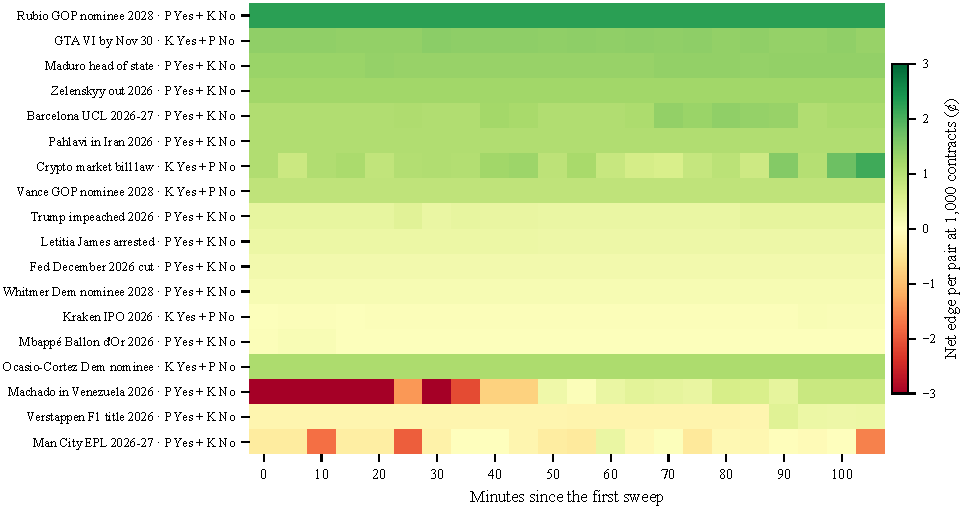
\includegraphics[width=\textwidth]{fig_free_timeline}
\caption{Net edge per pair on a \$1,000 bet for every free lunch in every sweep of the test. Green cells are positive; a free lunch that persists shows as an unbroken green row. The colour scale is clipped at $\pm 3$ cents.}\label{fig:timeline}
\end{figure*}

\begin{figure*}[t]
\centering
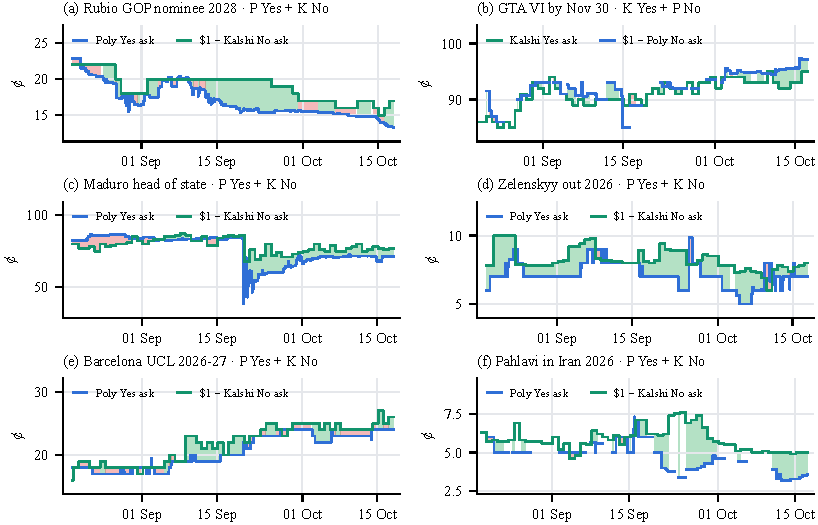
\includegraphics[width=\textwidth]{fig_free_history}
\caption{Ask histories of six free lunches over the last 60 days. Green hatching marks hours when the route cost less than a dollar after fees.}\label{fig:freehistory}
\end{figure*}

\subsection{The free lunches: evidence that they are real}

A free lunch has to pass five tests: the rules must match, the edge must be executable at size, it must persist, it must survive a re-check, and it should not be a one-off glitch in the history. Table~\ref{tab:evidence} collects the evidence for all 18. The rules test is the review above. The edge is computed from walked books after fees for all three bets. 14 of the 18 free lunches were positive at \$1,000 in all 22 sweeps (Fig.~\ref{fig:timeline}), and 348 of 349 re-checks a minute later were still positive. In the ask history the median free lunch was in the green 41\% of the time it could be observed, and 5 had been green for more than two weeks in a row at the end of the test (Fig.~\ref{fig:freehistory}).

Not every free lunch is equally solid. Verstappen F1 title 2026 and Man City EPL 2026-27 were positive in fewer than half of the sweeps and lost money on a \$1,000 bet in the median sweep. Fed December 2026 cut, Whitmer Dem nominee 2028 and Man City EPL 2026-27 had almost never been green in the history: these are gaps that open and close, not standing mispricings. Table~\ref{tab:rules} quotes the two rule texts for the three free lunches with the highest edge, so the match can be checked directly.

\begin{table}[tbp]
\caption{Settlement rules of the three free lunches with the highest edge on a \$1,000 bet, as published by each venue (opening words).}\label{tab:rules}
\footnotesize
\begin{tabularx}{\columnwidth}{@{}lL@{}}
\toprule
\multicolumn{2}{@{}l}{\textbf{Rubio GOP nominee 2028}} \\
Kalshi & If Marco Rubio wins and accepts the nomination for the Presidency for the Republican party in 2028, then the market resolves to Yes. \\
Polymarket & This market will resolve to ``Yes'' if the named individual wins and accepts the 2028 nomination of the Republican Party for U.S. president. Otherwise, this market will resolve to ``No''. \\
\midrule
\multicolumn{2}{@{}l}{\textbf{GTA VI by Nov 30}} \\
Kalshi & If GTA 6 (Grand Theft Auto VI) has been released on a major platform (PS5, Xbox Series X/S, Windows) by Nov 30, 2026, then the market resolves to Yes. \\
Polymarket & This market will resolve to ``Yes'' if it Grand Theft Auto VI is officially released in the US by the listed date, 11:59 PM ET. Otherwise, this market will resolve to ``No''. \\
\midrule
\multicolumn{2}{@{}l}{\textbf{Maduro head of state}} \\
Kalshi & If Nicol\'as Maduro officially holds the position of the head of state of Venezuela on Dec 31, 2026 at 10:00 AM ET, then the market resolves to Yes. \\
Polymarket & This market will resolve to the individual who officially holds the position of the head of state of Venezuela on Dec 31, 2026 at 12 PM ET. \\
\bottomrule
\end{tabularx}
\end{table}

\section{Discussion}\label{sec:discussion}

\subsection{The hypotheses}

Table~\ref{tab:hypotheses} sets each hypothesis against the evidence. Five are supported, H5 is supported for most of the free lunches but not all, and H7 is supported in the sense that matters for the money, with a clear exception for thin books.

\begin{table*}[t]
\caption{Hypotheses, evidence and verdict.}\label{tab:hypotheses}
\footnotesize
\begin{tabularx}{\textwidth}{@{}lLLl@{}}
\toprule
 & Hypothesis & Evidence & Verdict \\
\midrule
H1 & The pricing is reproduced by an independent implementation. & 736,856 values compared, 0 mismatches; 16 faults found, 14 fixed. & Supported \\
H2 & No single-market route costs less than \$1 after fees. & 0 of 13,882 single-market snapshots positive at \$1 or \$1,000; lowest ask sum 100.10\,\cent. & Supported \\
H3 & Some cross-market routes stay below \$1 after fees and depth at \$1,000. & 570 snapshots and 28 routes positive on a \$1,000 bet. & Supported \\
H4 & The largest apparent edges are not sure bets. & The three largest routes (3.66, 3.21, 2.99\,\cent) differ in settlement; median 1.10\,\cent{} against 0.64\,\cent{} for free lunches. & Supported \\
H5 & The free lunches persist. & 14 of 18 positive in all 22 sweeps; 348 of 349 re-checks positive; 5 green for more than two weeks; 2 positive in fewer than half the sweeps and 3 almost never green in the history. & Mostly supported \\
H6 & Cent rounding kills sub-cent free lunches on a \$1 bet; they pay above a few contracts. & Rounding cost a median 0.64\,\cent{} at \$1; 6 of 18 lost money; the 4 positive at \$1,000 in every sweep broke even at 2 to 6 contracts. & Supported \\
H7 & Books are deep enough for a \$1,000 bet without losing the edge. & All 18 had 1,000 contracts on both legs and 16 were profitable; 7 lost at least 0.3\,\cent{} to slippage, one from 5.65 to 0.15\,\cent. & Partly supported \\
\bottomrule
\end{tabularx}
\end{table*}

\subsection{Are the free lunches real?}

On the evidence available without trading, yes. Each one passed a reading of both rule books, was priced from the actual order books after both venues' fees, and stayed positive across sweeps and re-checks; the strongest had been visible in the ask history for weeks. The residual risks are of a different kind than market risk. The venues could interpret the same event differently, for example on the exact moment a nomination counts as accepted. The two legs are not filled at the same instant, so one could move before the other fills. A venue could change its fee schedule or restrict an account. Access is also subject to each platform's terms and to where the trader lives. A final proof would require filling both legs and holding them to settlement, which this study did not do.

\subsection{What bet size means for a trader}

The test gives three practical rules. First, do not bet small on Kalshi: below a few contracts the cent rounding can cost more than the edge, and on a leg priced near 1 or 99 cents it costs almost a full cent per order. Second, place each leg as one order. The rounding is charged per order, so a \$1,000 bet split into a thousand one-contract orders would pay it a thousand times and turn every sub-cent free lunch into a loss. Third, size the bet to the book, not to the budget. Up to the depth of the best levels the profit grows in proportion to the stake; beyond them every extra contract earns less, and on thin books such as the Machado route a \$1,000 bet captures almost nothing. Polymarket's 5-share minimum adds a floor of its own. Between those limits, in the range of a few dollars to about a thousand, the profit grows with the stake, which is where the free lunches in this test paid.

\subsection{Why do they persist?}

The edges are small and the money is locked up. The median free lunch earned 0.64 cents per pair on a \$1,000 bet and its markets settle 75 days after the test, which gives a median annualised return of about 1.2\%. The 2028 nomination markets tie capital for more than two years. Below a short-term interest rate, an arbitrage like this costs money to hold, which is the textbook limit to arbitrage \cite{shleifer1997,gromb2010}. A trader also needs funded accounts on two venues with different collateral, onboarding and jurisdictions. The size of the gaps, one to two cents on prices of 10 to 90 cents, is in line with the 2 to 4\% divergence that Gebele and Matthes \cite{gebele2026semantic} report across venues. The rounding adds a reason of its own: the many small traders who could close a sub-cent gap one contract at a time lose money doing it.

\subsection{Limitations and future work}\label{sec:limitations}

The forward test covers one window of under two hours on a weekend night, so it says nothing about how opportunities behave around news or during busy hours. The settlement review was done by one reader from the published rules; a second reader would make it stronger. The Polymarket ask history is rebuilt from trades rather than quotes and only reaches back 11,000 trades. Books were stored up to 1,000 contracts, so bets larger than about \$1,000 were not tested, and venue position limits were not checked. Finally, the matcher misses some true pairs (finding A7) and accepts some near pairs (A8). A practical fix for A7 is to skip the level-ratio test when the mean price gap is below three cents and to prefer the candidate with the closest deadline; for A8, to compare the dates named in both rule texts before accepting a pair. Both should be tested on the labelled sample before they are adopted. Future work: compare rule texts automatically, subscribe to order-book updates instead of polling, price multi-outcome events, and test execution with small orders on both venues.

\section{Conclusion}\label{sec:conclusion}

Prediction Engine matches 363 pairs across Kalshi and Polymarket and prices arbitrage at executable depth, and an independent implementation reproduced its pricing on 736,856 values (RQ1). Single-market arbitrage never appeared: the two asks of a market sum to a dollar plus the spread (RQ2). Cross-market routes did turn positive after fees, and reading the rules split the 28 flagged routes into 18 free lunches and 10 bets that only looked safe, which carried the largest edges (RQ3). Bet size decides whether a free lunch pays (RQ4). On a \$1 bet Kalshi's cent rounding wiped out six of them; above a few contracts the profit grew with the size of the bet, and on a \$1,000 bet 16 of 18 were profitable, while thin books cut the edge of a few. The practical lesson is that a scanner can find the gaps, the rules decide which ones are free, and the size of the bet decides how much of them a trader keeps.

\section*{Declaration of competing interest}

The author declares no competing financial interests. No positions were held in the markets studied.

\section*{Data availability}

The code is in the project repository. The forward-test snapshots, the settlement labels and the scripts that produce every figure and table are in the data folder that accompanies this report.

\section*{CRediT authorship contribution statement}

\textbf{Niclas Karlsen:} Conceptualization, Methodology, Software, Investigation, Formal analysis, Visualization, Writing.

\bibliographystyle{elsarticle-num}
\bibliography{references}

\onecolumn
\appendix

\section{The interface on two pairs}

Fig.~\ref{fig:uicross} shows the engine on the US aliens pair, a route that looks positive but is not a sure bet. Fig.~\ref{fig:uirubio} shows the cross-market chart and worksheet for the Rubio pair, with one column for a single contract and one for 1,000 contracts. Fig.~\ref{fig:uimath} shows the section of the interface that lists every formula of Section~\ref{sec:pricing} next to a worked example for the selected route. Numbers fetched from the venues are highlighted, so each step can be traced back to the order books.

\begin{figure}[htbp]
\centering
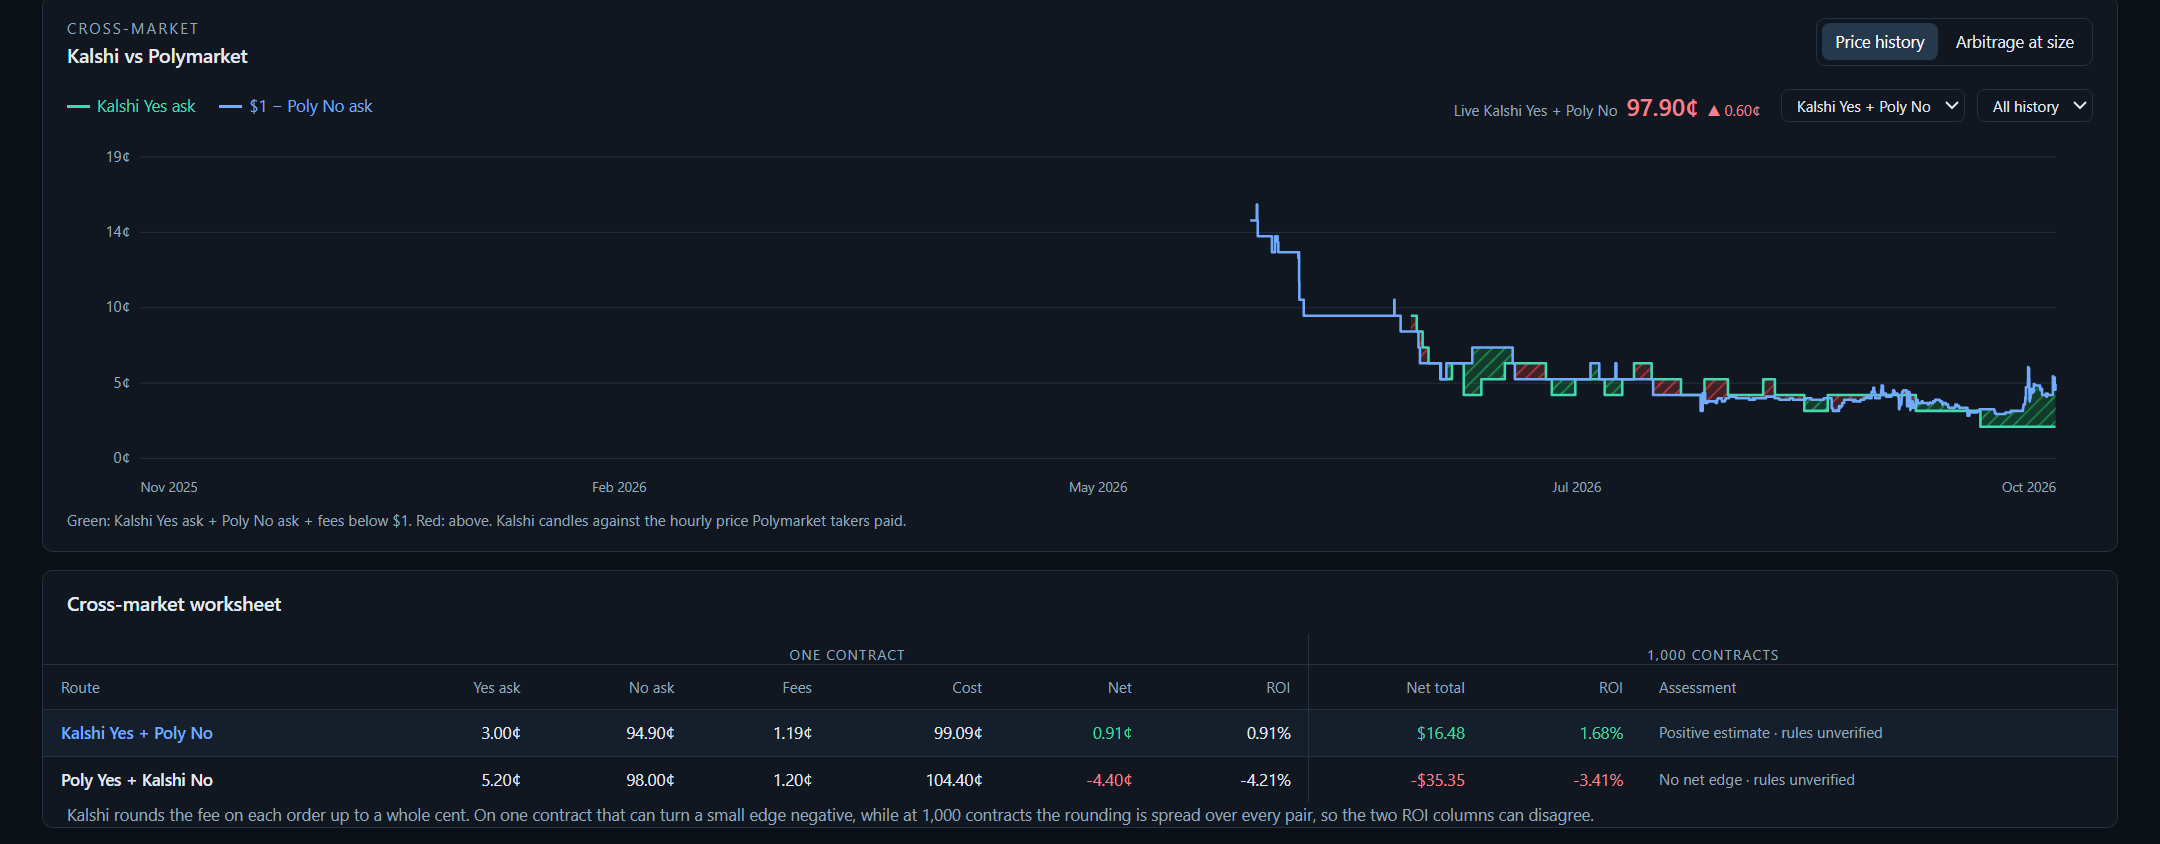
\includegraphics[width=0.8\textwidth]{ui_cross}
\caption{The engine on the US aliens pair. Kalshi Yes + Poly No is a positive estimate, but the Kalshi market closes on 1 December and the Polymarket market on 31 December, so the route is not a sure bet. The rules-unverified label is there for exactly this case.}\label{fig:uicross}
\end{figure}

\begin{figure}[htbp]
\centering
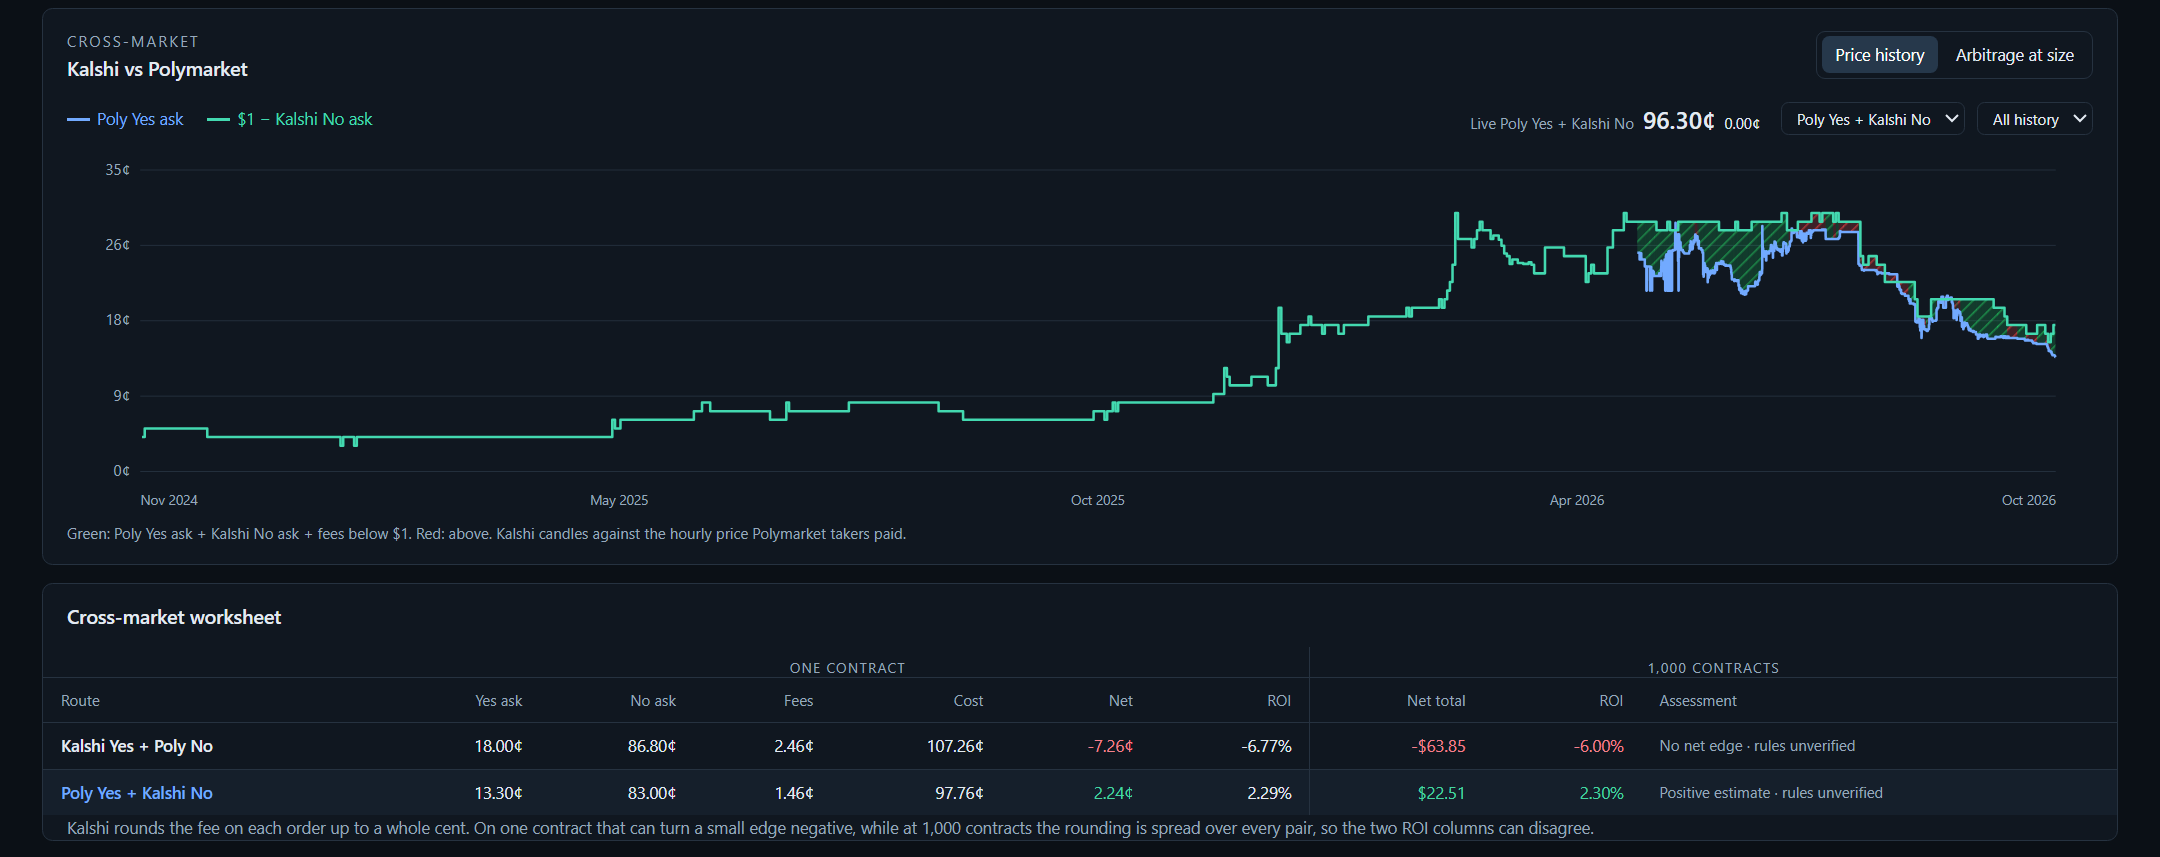
\includegraphics[width=0.85\textwidth]{ui_rubio_cross}
\caption{The cross-market chart and worksheet for the Rubio pair in the interface. The Poly Yes + Kalshi No route is a positive estimate for one contract and for 1,000 contracts; the ask history shows the same gap through most of the summer.}\label{fig:uirubio}
\end{figure}

\begin{figure}[htbp]
\centering
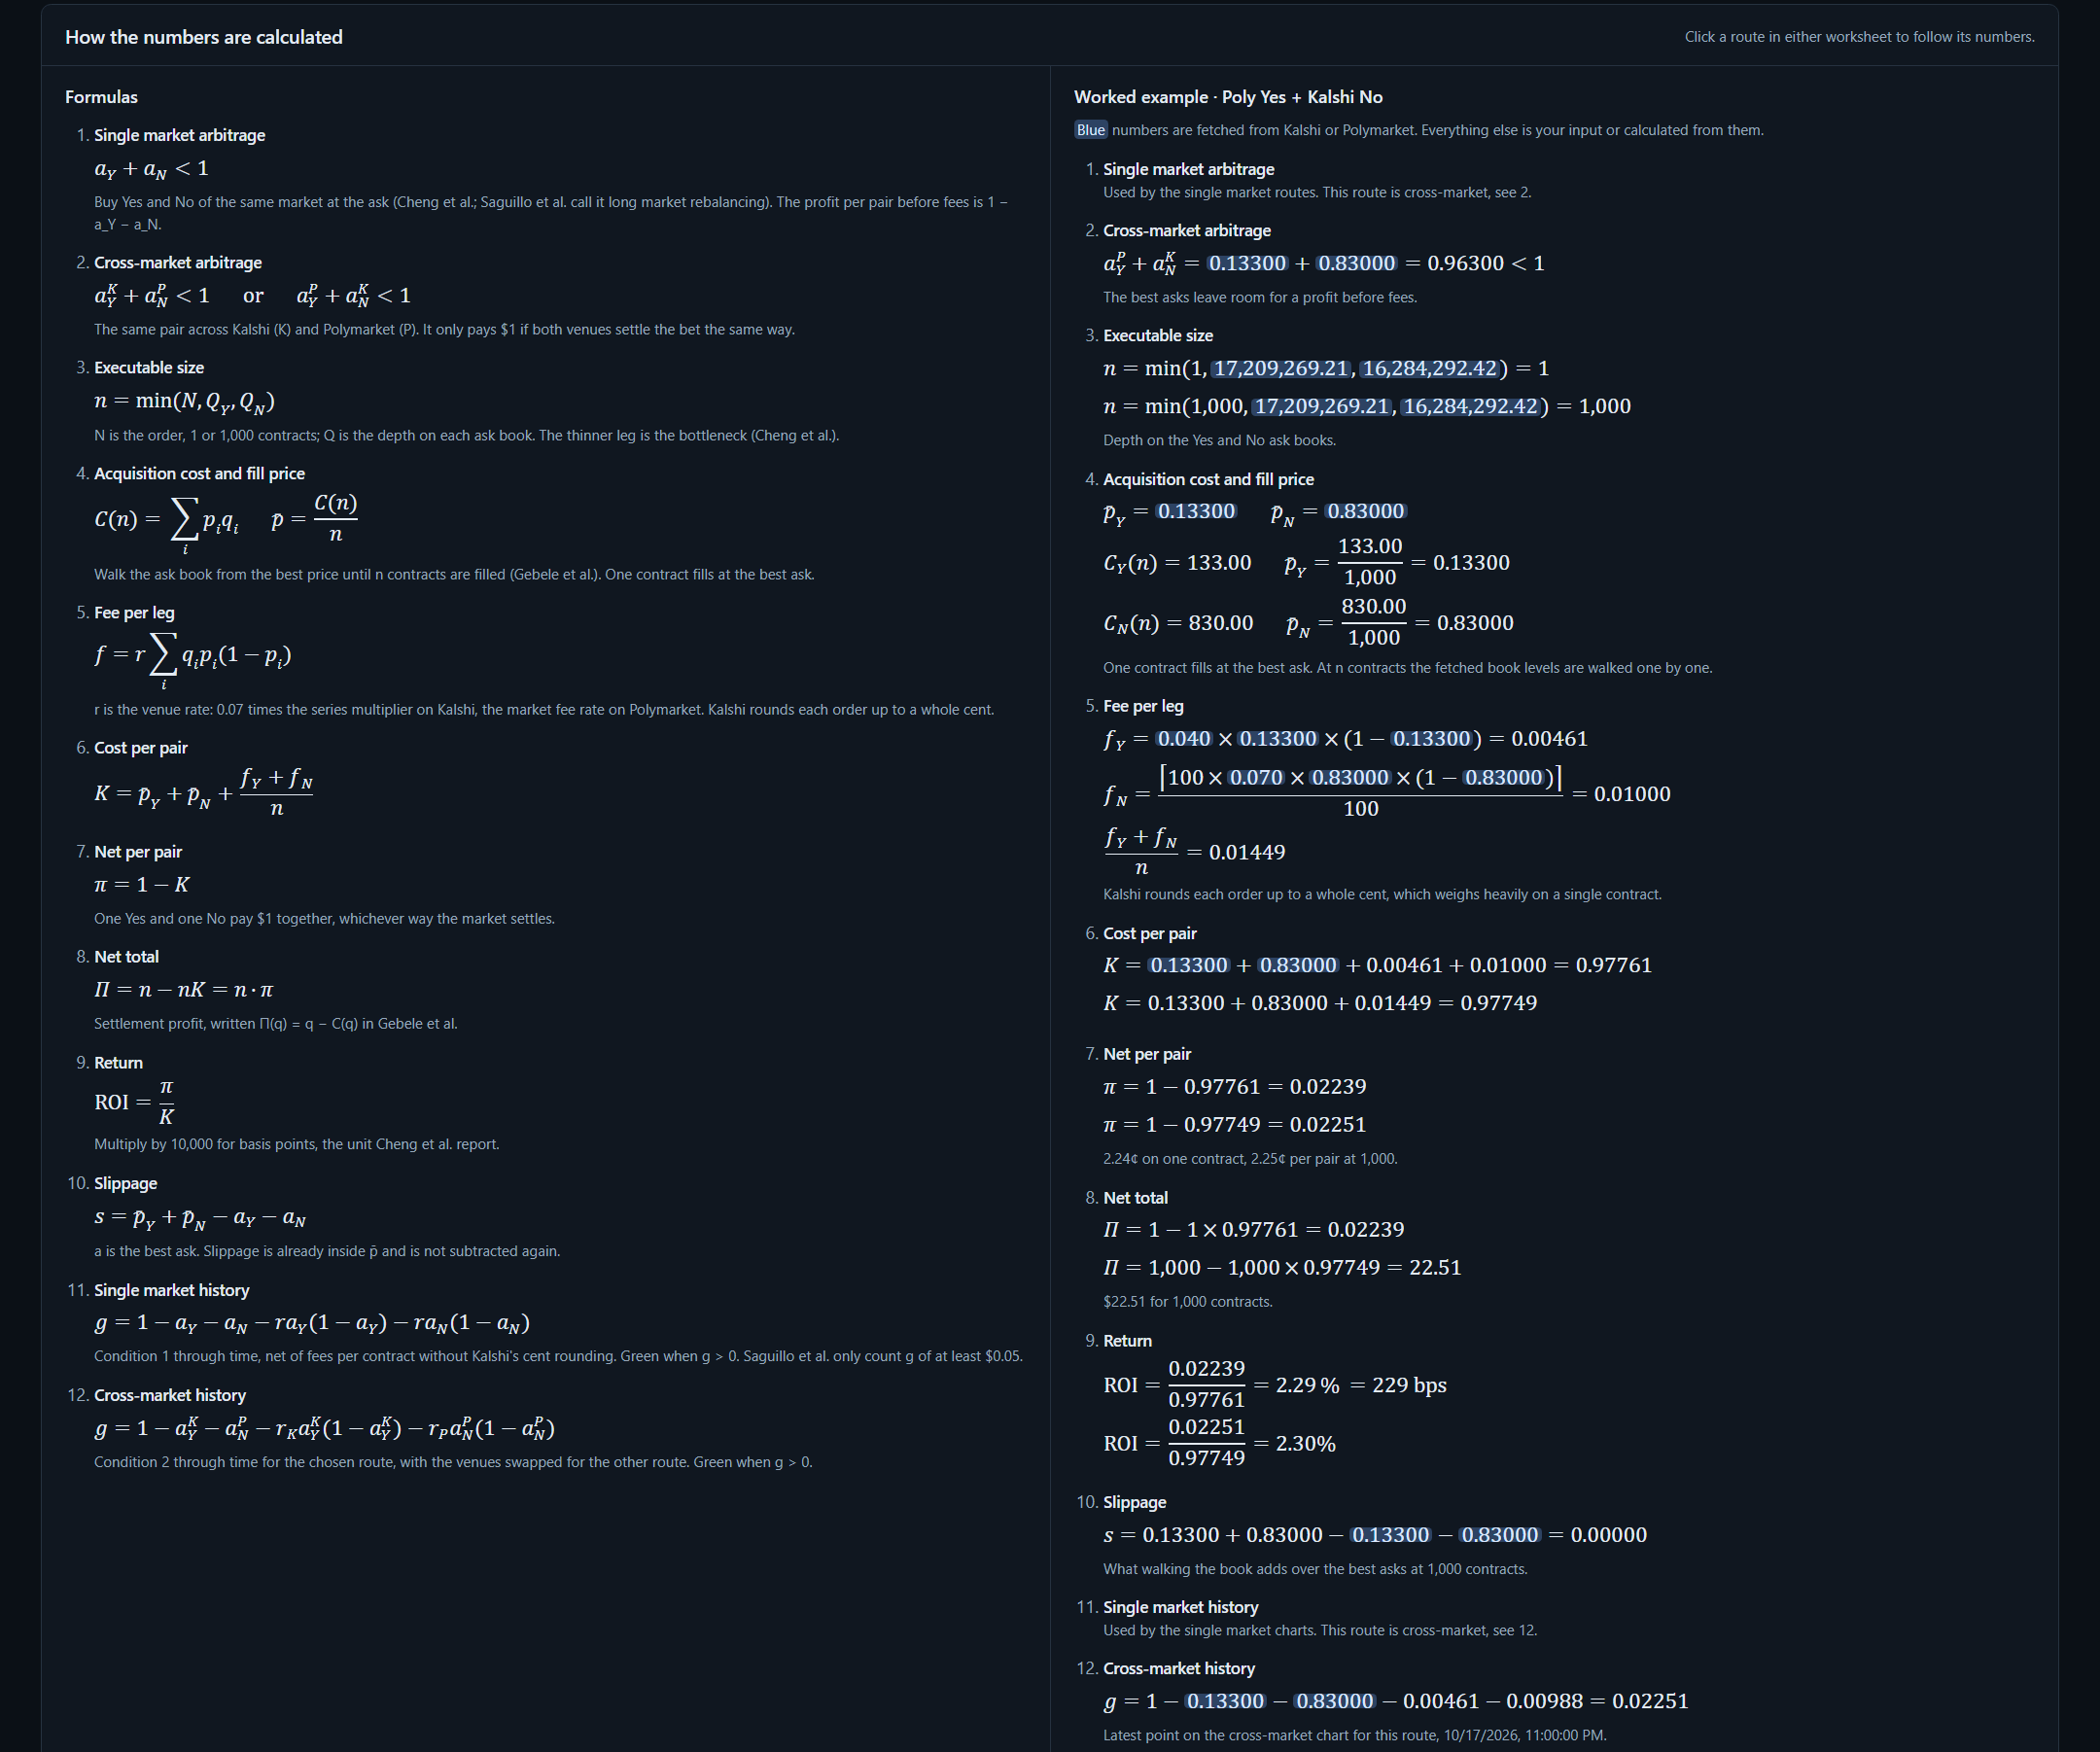
\includegraphics[width=0.85\textwidth]{ui_rubio_math}
\caption{Formulas and the worked example for Poly Yes + Kalshi No on the Rubio pair, as shown in the interface.}\label{fig:uimath}
\end{figure}

\end{document}
